\documentclass[conference]{IEEEtran}
\IEEEoverridecommandlockouts
%----------------------------------------------------------
%\graphicspath{images/}
%\DeclareGraphicsExtensions{.pdf,.jpeg,.png,.jpg}
\usepackage{amsmath,amssymb,amsfonts}
\usepackage{algorithmic}
\usepackage{graphicx}
\usepackage{textcomp}
\usepackage{array}
%\usepackage[caption=false,font=normalsize,labelfont=sf,textfon =sf]{subfig}
\usepackage{dblfloatfix}
\usepackage{url}
\usepackage{lipsum}
\usepackage{listings}
\usepackage{xcolor}
\def\BibTeX{{\rm B\kern-.05em{\sc i\kern-.025em b}\kern-.08em
    T\kern-.1667em\lower.7ex\hbox{E}\kern-.125emX}}
%----------------------------------------------------------
\lstset{
    escapeinside={/*@}{@*/},
    language=Python,	
    basicstyle=\fontsize{8.5}{12}\selectfont,
    numbers=left,
    numbersep=2pt,    
    xleftmargin=2pt,
    frame=tb,
    columns=fullflexible,
    showstringspaces=false,
    tabsize=4,
    keepspaces=true,
    showtabs=false,
    showspaces=false,
    morekeywords={inline,public,class,private,protected,struct},
    captionpos=b,
    lineskip=-0.4em,
    aboveskip=10pt,
    extendedchars=true,
    breaklines=true,
    prebreak = \raisebox{0ex}[0ex][0ex]{\ensuremath{\hookleftarrow}},
    keywordstyle=\color[rgb]{0,0,1},
    commentstyle=\color[rgb]{0.133,0.545,0.133},
    stringstyle=\color[rgb]{0.627,0.126,0.941},
}
%----------------------------------------------------------
\begin{document}

\title{Desafio 2: Sistema Embarcado com Sensor e Display\\
{\footnotesize Sistemas Embarcados: Prof. Marco Reis - marco.reis@ba.docente.senai.br}
}

\author{\IEEEauthorblockN{Leonardo Marques Trinchão}
\IEEEauthorblockA{\textit{Senai CIMATEC} \\
\textit{Engenharia Elétrica}\\
Salvador, Bahia, Brazil \\
leonardo.trinchao@aln.senaicimatec.edu.br}
}

\maketitle

\begin{abstract}

\end{abstract}
    
\begin{IEEEkeywords}
    component, formatting, style, styling, insert
\end{IEEEkeywords}
    
\section{Introdução}
\subsection{Arduino}

    Arduino é uma plataforma de prototipagem eletrônica, cujo principal objetivo é incorporar a ele 
funções através de componentes como sensores, LED's, módulos, e outros. A partir disso, torna-se 
possível criar sistemas embarcados versáteis para projetos em eletrônica, que consistem em criar desde 
pequenos robôs com funções limitadas, até protótipos baseados na utilização de Internet das Coisas (IoT),
automações residenciais, e outros.

    Para realizar as ações desejadas pelo usuário, é necessário programar o Arduino. Para isso, utiliza-se 
a linguagem de programação C/C++. Após ser programado, ele funciona sem a necessidade de um computador, por
exemplo, devido à um \emph{loop} que existe em seu próprio código. Assim, a única exigência para o
funcionamento do sistema é que haja uma fonte de alimentação.

    É possível identificar abaixo como é a representação de um Arduíno UNO, utilizado no projeto, através
da Fig.~\ref{fig}.

\begin{figure}[htbp]
    \centerline{
        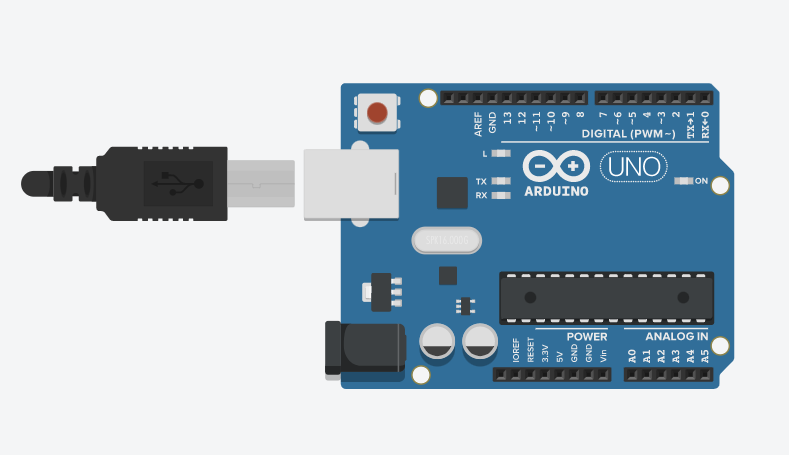
\includegraphics[width=8cm]{images/Arduino_UNO.png}
        }
    \caption{Exemplo de um Arduino UNO.}
    \label{fig}
    \end{figure}

\subsubsection{Arduino Pricipal}

    O Arduino Principal/Arduino Master recebe este nome devido à sua importância e relevância no projeto.
Ele recebe este nome por ser o responsável por controlar todo o sistema embarcado, de forma que realiza
cálculos matemáticos, operações e comandos envolvendo bibliotecas do próprio Arduino.

\subsubsection{Arduino Secundário}

    O Arduino Secundário/Arduino Slave é um sistema microprocessado que atua como suporte para o 
Arduino Master, ou seja, sua função é complementar suas necessidades, de acordo com o que é exigido.
Para que esse suporte seja realizado com êxito, é necessário comunicar os dois Arduinos, e para isso
utiliza-se a Comunicação Serial.

\subsection{Comunicação Serial}

    É possível que, em um sistema, dois Arduinos exerçam um papel complementar, onde um não funciona
perfeitamente sem o outro. Para sintonizar os dois Arduinos, é necessário criar um meio de Comunicação
entre eles, e com isso surge a Comunicação Serial. Ela funciona de forma que um Arduino Principal realiza
a principal parte do código, e pode existir um ou mais Arduinos Complementares, que exercem, como o próprio
nome diz, funções complementares.

    A partir disso, o Arduino Principal envia uma informação, seja ela um valor inteiro, uma letra ou uma
\emph{string}, e o(s) Arduino(s) Complementar(es) recebem essa informação e a utilizam para realizar suas
demais funções, como exibir essa informação em um \emph{LCD Display}. 

    Para que essa comunicação seja possível, é necessário realizar alguns procedimentos antes, como:
    \begin{itemize}
        \item Conectar as portas TX (transmissão) e RX (recepção) dos Arduinos;
        \item Conectar as portas \emph{Ground} dos Arduinos;
        \item Uso da biblioteca \emph{SoftwareSerial.h} nos dois Arduinos;
        \item Uso do comando \emph{Serial.begin(9600)} dentro da \emph{void setup}, também nos dois;
        \item Uso de condição envolvendo \emph{Serial.available()} no Arduino Complementar;
        \item Receber o valor impresso no monitor serial do Arduino Pricipal utilizando 
        \emph{Serial.readString()};
        \item Atribuir esse valor à uma variável do tipo \emph{String};
        \item Utilizar o comando \emph{Serial.flush()} para esperar toda a "passagem" da informação.
    \end{itemize}

\subsection{Sensor Ultrassônico}

    O Sensor Ultra-Sônico é um componente utilizado no Arduino para captar a distância de um objeto, 
entre os pontos de mínimo e máximo, de acordo com a capacidade do sensor. O ponto de distância mínima 
é de aproximadamente 3 centímetros, e o ponto de alcance máximo é de 330 centímetros. Ele é muito
utilizado em indústrias, para detectar a posição de materiais granulados, fluidos e materiais em pó.
O sensor capta o tempo e a velocidade de propagação das ondas ultrassônicas, e torna possível encontrar
a distância.

É possível identificar abaixo como é a representação de um Sensor Ultrassônico, utilizado no projeto, 
através da Fig.~\ref{fig}.

\begin{figure}[htbp]
    \centerline{
        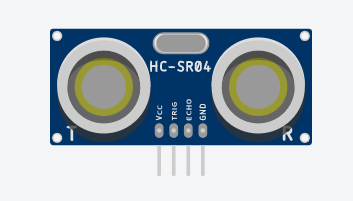
\includegraphics{images/Sensor.png}
        }
    \caption{Exemplo de um Sensor Ultrassônico.}
    \label{fig}
    \end{figure}

\subsection{LED RGB}

    O LED RGB se diferencia dos LED's tradicionais pelo fato de poder utilizar diferentes tonalidades de
vermelho, verde e azul, a fim de se obter uma cor diferente. Seu uso pode otimizar o código e torná-lo
mais prático, visto que utiliza-se apenas um LED que pode representar as três cores, ao invés de 3 com
cores específicas.

É possível identificar abaixo como é a representação de um LED RGB, utilizado no projeto, através
da Fig.~\ref{fig}.

\begin{figure}[htbp]
    \centerline{
        
\includegraphics{images/LED_RGB.png}
        }
    \caption{Exemplo de um LED RGB.}
    \label{fig}
    \end{figure}

\subsection{Liquid Crystal Display (LCD)}

    Ao utilizar um Arduino para realizar um cálculo ou uma operação, surge a possibilidade de exibir essa
informação na tela de um LCD Display. Ele é formado por uma tela fina, com tamanho 16x2, e possui a mesma
tecnologia utilizada em antigos televisores e monitores, sendo diferenciado pela sua leveza e praticidade.

É possível identificar abaixo como é a representação de um Display 16x2, utilizado no projeto, através
da Fig.~\ref{fig}.

\begin{figure}[htbp]
    \centerline{
        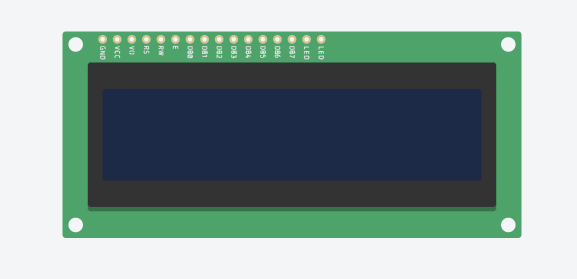
\includegraphics[width=8cm]{images/Display.png}
        }
    \caption{Exemplo de um Display 16x2.}
    \label{fig}
    \end{figure}

\section{Objetivos}

    O projeto apresentado tem como objetivo criar um sistema capaz de reconhecer um obstáculo/objeto,
reconhecer sua distância, identificar qual região se encontra e exibir essas informações em uma tela de 
display. Para isso, foram utilizados dois Arduinos, um para realizar o reconhecimento do objeto, computar
sua distância e acender um LED com a cor da região, e outro para exibir essas informações utilizando o
LCD. Para comunicar os Arduinos, foi utilizada a comunicação serial.

\section{Resultados}

    O projeto foi realizado através da platadorma \emph{Tinkercad}, que disponibiliza todos os materiais
necessários para a confecção do sistema apresentado. Para montar o projeto. foram utilizados os seguintes
materiais:
    \begin{itemize}
        \item 2 Arduinos Uno R3, sendo um Master e um Slave;
        \item 1 LCD 16x2;
        \item 1 Sensor de distância Ultrassônico;
        \item 4 Resistores de 220 Ohm;
        \item 1 LED RGB.
    \end{itemize}

    Primeiramente, o Arduino Principal (ou Arduino Master) exerce o papel de armazenar o "cérebro" do 
projeto. É nele que se configura o sensor, manipulando as portas ECHO e TRIG (portas de recepção e 
transmissão de sinais, respectivamente). Além disso, também configura o LED RGB, e faz o cálculo da 
distância que o objeto está do sensor. Para fazer o cálculo, utiliza-se a velocidade e o tempo captado 
pelo sensor, através da equação abaixo:

    \begin{equation}
        S=v.t \label{eq}
    \end{equation}

    Na equação \eqref{eq}, \emph{S} representa a distância que deseja-se obter, \emph{v} é a velocidade
de propagação da onda do sensor ultrassônico, previamente calculado, cujo valor é de \emph{0,017175}, e
o \emph{t} é o tempo dessa propagação, calculado através do pulso da porta ECHO.

    Tratando-se das regiões do sensor,  partindo da distância mínima do sensor, que equivale a
3 centímetros até 110 centímetros (1/3 da distância) tem-se a Região 3. Partindo de 110 até 220 
centímetros (2/3 da distância), tem-se a Região 2, e de 220 até 330 centímetros	tem-se a Região 1,
definida como a região mais distante do sensor.

    Ademais, para o LED funcionar, é necessário criar funções que representam cada cor, sendo elas 
vermelho, verde e azul. Como no projeto a cor amarela foi utilizada, é necessário unir as cores vermelho
e verde para obtê-la. Dessa forma, para acender o LED da cor desejada, de acordo com a região do objeto,
criou-se uma condição dentro da programação do Arduino, que dintingue essa região e aciona o LED da 
cor desejada.

    Além disso, o projeto exibe tanto a informação acerca da região do objeto, quanto o valor da distância
encontrada. Isso acontece em outro Arduino, chamado de Arduino Complementar ou Arduino Slave, que recebe
a informação transmitida pelo Arduino Master através da comunicação serial, e mostra, por exemplo,
a seguinte mensagem: \emph{"REGIAO 2: 133.66}. Isso significa que o objeto se encontra na região 2, 
ou seja, a "zona intermediária" do sensor, e o valor que segue é a distância, dada em centímetros, além
da LED exibir a coloração amarela.

    É evidente que o sistema não funciona apenas com os códigos e a montagem do esquemático, devem existir
conexões entre as portas dos Arduinos com os componentes utilizados. Para isso, tem-se que o sensor fica 
atrelado às portas digitais do Arduino Master, à porta de 5 Volts e ao \emph{ground} "GRD", que representa
o fio terra. A LED também está conectada às portas digitais e ao GRD. Por fim, no Arduino Master, também
existe a conexão feita com o Arduino Slave, através das portas RX e TX, ambas já citadas no relatório.

    Tratando-se do Arduino Slave, têm-se como conexões, além das portas TX e RX, as portas digitais D8 até
a D13 atreladas ao LCD, juntamente com o GRD e a porta de 5 Volts. Também existe um resistor de 220 Ohm para
evitar a sobrecarga no \emph{display}.

Abaixo na Fig.~\ref{fig}, é possível visualizar a forma esquemática de como o projeto está 
representado, utilizando todos os elementos citados no relatório, além de fios de conexão.

\begin{figure}[htbp]
    \centerline{
        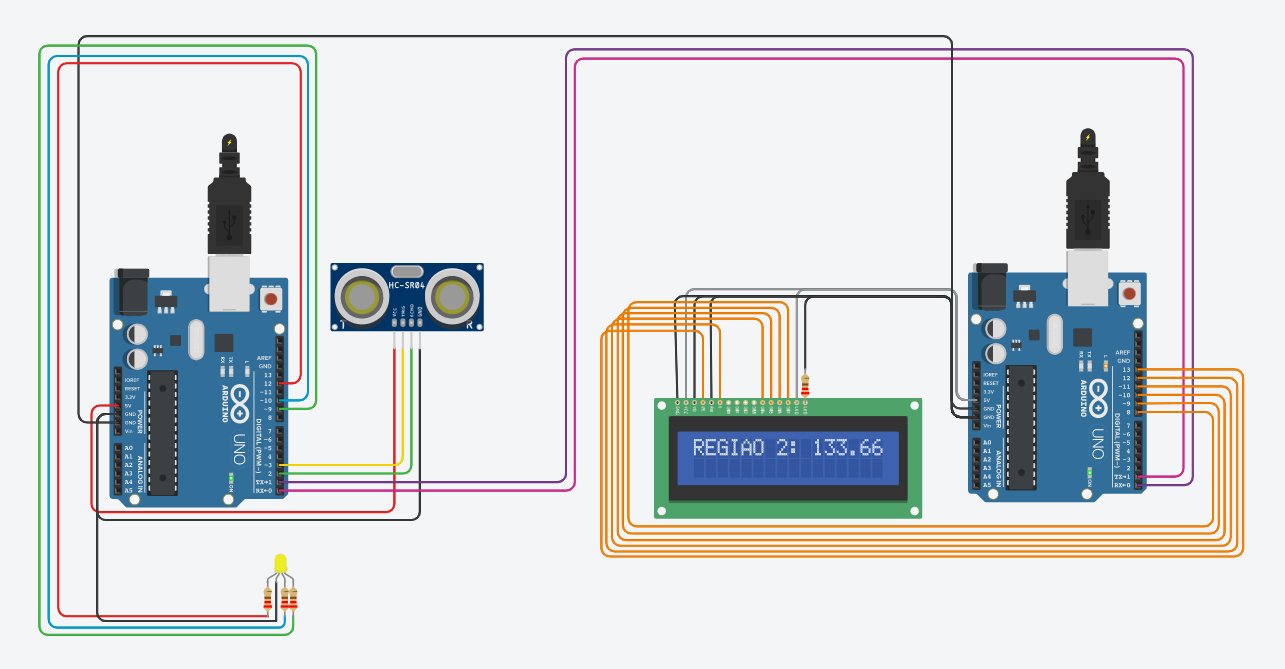
\includegraphics[width=8cm]{images/esquematico.png}
        }
    \caption{Esquemático do projeto.}
    \label{fig}
    \end{figure}

\section{Referências}

\end{document}